\cleardoubleoddpage
\chapter{Corpus--Generator Analysis with Statistical Support}
\label{chap:main-results}

%% Draft preamble note (kept in source for reference; not rendered):
%% Written to be read by the thesis supervisor first, then polished into
%% final prose. All quantitative claims trace back to a specific Entry
%% in docs/THESIS_FINDINGS_LOG.md and to a specific committed bootstrap
%% script under scripts/.


\section{Chapter overview}
\label{sec:main-results-overview}

This chapter presents the main empirical results of the thesis. It
addresses three of the four research questions stated in the
writing plan:

\begin{itemize}
    \item \textbf{RQ1 --- Does dialectal / domain-shifted speech affect deepfake
        detection performance?} Answered by comparing the primary
        detector's error rate on Tyneside DECTE audio against its error
        rate on a standard-accent VCTK control set, holding the generator
        fixed (Sections~\ref{sec:main-results-aasist-xtts},~\ref{sec:main-results-aasist-openvoice}).
    \item \textbf{RQ2 --- Does the effect of dialect / domain shift interact with
        the choice of spoof generator?} Answered by running the same
        DECTE-vs-VCTK comparison for a second generator (OpenVoice v2)
        and comparing the outcome to the XTTS v2 outcome (Section~\ref{sec:main-results-aasist-openvoice}).
    \item \textbf{RQ4 --- Do the main corpus-gap patterns persist across detector
        architectures?} Answered by re-running the whole XTTS and
        OpenVoice comparison with a completely different detector family
        (LFCC + Logistic Regression) and checking whether the direction
        and magnitude of the gaps agree (Sections~\ref{sec:main-results-lfcc-xtts},~\ref{sec:main-results-lfcc-openvoice}).
\end{itemize}

Every headline number in this chapter is reported with a 95\,\%
non-parametric bootstrap confidence interval, computed via the
protocol laid out in Chapter~\ref{chap:data-methodology}, Section~\ref{sec:methodology-bootstrap} (1000 iterations,
seed 42, joint per-corpus resampling for gap CIs). The chapter is
descriptive of the results themselves; the framing of what these
results mean for the thesis' broader questions is expanded in
Chapter~\ref{chap:discussion} (Discussion \& Limitations).

This chapter carries the central evidence of the thesis. It does
more than report detector error rates: it shows that the direction
of the corpus gap depends on the spoof generator. That is why the
XTTS and OpenVoice results are reported separately before being
combined in the final $2 \times 2$ table.


\section{Result structure}
\label{sec:main-results-design}

The main analysis in this chapter is organised around a small
factorial structure --- two corpora, two generators, two detectors ---
that produces eight distinct evaluation cells:

\begin{itemize}
    \item \textbf{Two corpora}: DECTE (Tyneside dialectal / interview-style
        speech) and VCTK 0.92 (loose English-accent studio-read speech,
        20-speaker slate). The corpus preparation and speaker selection
        are described in Chapter~\ref{chap:data-methodology}, Section~\ref{sec:methodology-corpora}.
    \item \textbf{Two generators}: XTTS v2 (Coqui, end-to-end zero-shot cloning)
        and OpenVoice v2 (MyShell, base TTS + tone-colour converter).
        Both are described in Chapter~\ref{chap:data-methodology}, Section~\ref{sec:methodology-spoof-generation}.
    \item \textbf{Two detectors}: the primary AuralGuard-AASISTPP wrapper around
        AASIST (Chapter~\ref{chap:data-methodology}, Section~\ref{sec:methodology-detectors-aasist}; verified in Chapter~\ref{chap:detector-verification}) and a
        secondary LFCC + Logistic Regression classifier (Chapter~\ref{chap:data-methodology},
        Section~\ref{sec:methodology-detectors-lfcc-lr}), used specifically as a cross-architecture
        replication check.
\end{itemize}

Each of the eight cells is scored by exactly one detector on
exactly one (corpus, generator) audio slice. All 100-spoof VCTK
counts and all 216 / 86 / 120 bonafide counts (whichever applies)
follow the matched-N and matched-pair evaluation protocol of
Chapter~\ref{chap:data-methodology}, Section~\ref{sec:methodology-evaluation-protocol}. The bootstrap machinery of Section~\ref{sec:methodology-bootstrap} is
what turns each cell's EER point estimate into a 95\,\% CI, and each
DECTE-vs-VCTK comparison into a CI on the corpus gap itself.

The chapter reports the cells in a fixed order:

\begin{enumerate}
    \item AASIST + XTTS (Section~\ref{sec:main-results-aasist-xtts}) --- the primary dialect / domain-gap
        result.
    \item LFCC + LR + XTTS (Section~\ref{sec:main-results-lfcc-xtts}) --- the cross-architecture
        replication of the XTTS gap.
    \item AASIST + OpenVoice (Section~\ref{sec:main-results-aasist-openvoice}) --- the generator-dependent
        reversal result.
    \item LFCC + LR + OpenVoice (Section~\ref{sec:main-results-lfcc-openvoice}) --- the cross-architecture
        replication of the OpenVoice reversal.
    \item A combined $2 \times 2$ (corpus $\times$ generator) $\times$ 2 (detector) table
        (Section~\ref{sec:main-results-combined}).
    \item Answers to RQ1, RQ2, RQ4 (Section~\ref{sec:main-results-rq-answers}) and limitations of the
        chapter's evidence (Section~\ref{sec:main-results-limitations}).
\end{enumerate}


\section{AASIST XTTS corpus gap --- the primary dialect / domain-gap result}
\label{sec:main-results-aasist-xtts}

The primary dialect / domain-gap comparison holds the detector and
the generator fixed and varies only the corpus. Under the primary
detector (AuralGuard-AASISTPP, baseline checkpoint verified in
Chapter~\ref{chap:detector-verification}) and XTTS v2, the DECTE arm was evaluated against the
DECTE bonafide pool of 216 unique matched originals; the VCTK arm
was evaluated against the VCTK bonafide pool of 120 unique matched
originals. Both arms use 100 XTTS v2 spoofs --- for the DECTE arm this
is a stratified random subsample from the full 416-spoof pool
(seed 42), for the VCTK arm this is the full XTTS pool from the
Entry 5 run. This matched-N protocol is what makes the two per-%
corpus point estimates directly comparable.

The point estimates and 95\,\% non-parametric bootstrap confidence
intervals are:

\begin{table}[t]
\centering
\caption{AASIST XTTS v2 per-corpus EER with 95\,\% bootstrap CIs.}
\label{tab:main-results-aasist-xtts}
\begin{tabularx}{\linewidth}{X r r r c r}
\toprule
\textbf{Arm} & \textbf{$n_\text{bonafide}$} & \textbf{$n_\text{spoof}$} & \textbf{EER (\%)} & \textbf{95\,\% CI (\%)} & \textbf{AUC} \\
\midrule
DECTE XTTS v2 & 216 & 100 & 34.63 & 28.85--41.33 & 0.6792 \\
VCTK XTTS v2  & 120 & 100 & 21.83 & 15.91--27.25 & 0.8917 \\
\bottomrule
\end{tabularx}
\end{table}

The DECTE-minus-VCTK gap is \textbf{$+12.80$ percentage points, with 95\,\%
bootstrap CI $[+6.13, +22.07]$\,pp}. The full CI lies above zero.
This is the primary quantitative result behind RQ1: with the
detector and generator held fixed, the corpus difference between
Tyneside DECTE and standard-accent VCTK produces a statistically
supported difference in detector error rate at 95\,\%.

Two things are worth flagging about the way this is stated:

\begin{itemize}
    \item The gap is a \textbf{corpus / domain gap}, not a pure dialect gap.
        DECTE and VCTK differ on multiple axes simultaneously (dialect,
        recording style, channel, age distribution --- see Section~\ref{sec:main-results-limitations}).
        The observed $+12.80$\,pp point estimate cannot be attributed
        exclusively to the dialect axis.
    \item The gap is a \textbf{95\,\% result under the specific detector-and-%
        generator pairing used here}. What happens under other detectors
        is the subject of Section~\ref{sec:main-results-lfcc-xtts} (LFCC + LR); what happens under
        other generators is the subject of Section~\ref{sec:main-results-aasist-openvoice} (OpenVoice).
        Neither of those questions is answered by Section~\ref{sec:main-results-aasist-xtts} alone.
\end{itemize}

Reproducer: \texttt{scripts/06\_bootstrap\_xtts\_corpus\_gap.py} (bootstrap on
predictions from \texttt{results/detector\_predictions.csv} and
\texttt{results/vctk/detector\_predictions.csv}, no rescoring). Details are
in Entry 6 of the findings log.


\section{LFCC + LR XTTS replication --- cross-architecture check}
\label{sec:main-results-lfcc-xtts}

To test whether the corpus gap reported in Section~\ref{sec:main-results-aasist-xtts} is specific
to the AASIST architecture, the same DECTE-vs-VCTK XTTS comparison
was repeated on a hand-crafted-feature LFCC + Logistic Regression
detector. The two detectors differ on nearly every architecturally
meaningful axis --- feature representation (learned vs hand-crafted),
model family (deep graph-attention vs convex linear), and
optimisation regime (SGD with dropout vs LBFGS on a small feature
matrix) --- so a same-direction gap on both detectors is not
architecture-specific in any straightforward sense.

The LFCC + LR classifier was fitted on the AuralGuard training CSV
with the 16 DECTE mitigation-test speakers filtered out
(Chapter~\ref{chap:data-methodology}, Section~\ref{sec:methodology-detectors-lfcc-lr}), then evaluated on the same audio files
as the AASIST detector's XTTS eval. The point estimates and
95\,\% bootstrap CIs are:

\begin{table}[t]
\centering
\caption{LFCC + LR XTTS v2 per-corpus EER with 95\,\% bootstrap CIs.}
\label{tab:main-results-lfcc-xtts}
\begin{tabularx}{\linewidth}{X r r r c r}
\toprule
\textbf{Arm} & \textbf{$n_\text{bonafide}$} & \textbf{$n_\text{spoof}$} & \textbf{EER (\%)} & \textbf{95\,\% CI (\%)} & \textbf{AUC} \\
\midrule
DECTE XTTS v2 (LFCC + LR) & 216 & 100 & 44.19 & 36.05--51.16 & 0.6605 \\
VCTK XTTS v2 (LFCC + LR)  & 120 & 100 & 31.75 & 25.00--38.17 & 0.7262 \\
\bottomrule
\end{tabularx}
\end{table}

The DECTE-minus-VCTK gap is \textbf{$+12.44$ percentage points, with 95\,\%
bootstrap CI $[+1.96, +21.76]$\,pp}. The full CI lies above zero.

Two features of this replication are directly meaningful for the
thesis' argument:

\begin{itemize}
    \item \textbf{Same direction.} Both detectors show DECTE $>$ VCTK. The sign
        of the gap is invariant across the two architectures tested.
    \item \textbf{Similar magnitude.} The AASIST gap ($+12.80$\,pp) and the
        LFCC + LR gap ($+12.44$\,pp) differ by about a third of a
        percentage point. Given the bootstrap CIs of $\sim$$\pm 10$\,pp on each
        arm, this is well within sampling noise --- the two point
        estimates are consistent with a common underlying corpus-gap
        effect on the order of $\sim$10--13\,pp.
\end{itemize}

The two detectors do not agree on the absolute EER level (LFCC +
LR is a weaker classifier overall --- its DECTE EER is $\sim$10\,pp above
the AASIST DECTE EER, and its VCTK EER is $\sim$10\,pp above the AASIST
VCTK EER). The magnitude of the \emph{gap}, however, is nearly the same
in both cases. That is the property Chapter~\ref{chap:main-results} leans on.

Reproducer: \texttt{scripts/11\_lfcc\_lr\_second\_detector.py} (fits the LFCC +
LR classifier and runs the bootstrap in a single self-contained
run). Details are in Entry 8 of the findings log.


\section{AASIST OpenVoice reversal --- direction depends on generator}
\label{sec:main-results-aasist-openvoice}

The primary detector was then evaluated on the second generator
(OpenVoice v2) under the same DECTE-vs-VCTK protocol. The DECTE arm
used the 100 OpenVoice v2 spoofs against the full 216-row DECTE
bonafide pool; the VCTK arm used 100 OpenVoice v2 spoofs against
the 120-row VCTK bonafide pool. All eight cell-level counts are
identical to Section~\ref{sec:main-results-aasist-xtts}, only the generator differs.

The point estimates and 95\,\% bootstrap CIs are:

\begin{table}[t]
\centering
\caption{AASIST OpenVoice v2 per-corpus EER with 95\,\% bootstrap CIs.}
\label{tab:main-results-aasist-openvoice}
\begin{tabularx}{\linewidth}{X r r r c r}
\toprule
\textbf{Arm} & \textbf{$n_\text{bonafide}$} & \textbf{$n_\text{spoof}$} & \textbf{EER (\%)} & \textbf{95\,\% CI (\%)} & \textbf{AUC} \\
\midrule
DECTE OpenVoice v2 & 216 & 100 & 47.84 & 41.83--53.39 & 0.5675 \\
VCTK OpenVoice v2  & 120 & 100 & 74.58 & 68.17--80.92 & 0.1643 \\
\bottomrule
\end{tabularx}
\end{table}

The DECTE-minus-VCTK gap is \textbf{$-26.74$ percentage points, with 95\,\%
bootstrap CI $[-35.69, -18.26]$\,pp}. The full CI lies below zero.

This is the second central quantitative result of the
chapter, and it goes in the opposite direction from Section~\ref{sec:main-results-aasist-xtts}.
Under the same detector, the same bonafide pools, the same audio
preprocessing, and the same evaluation protocol, OpenVoice v2
spoofs produce a \emph{lower} EER on DECTE than on VCTK. The dialect /
domain axis that made XTTS harder on DECTE (Section~\ref{sec:main-results-aasist-xtts}) does not
merely have a smaller effect for OpenVoice --- it appears to run in
the opposite direction.

Interpreted structurally, this rules out an explanation in which
DECTE is uniformly ``harder'' than VCTK for anti-spoofing
regardless of what is being detected. If DECTE were uniformly
harder, then holding the detector fixed and swapping the generator
would preserve the sign of the gap --- it would only shift its
magnitude. The observed sign flip means the interaction between
generator and corpus is doing real work: for the OpenVoice v2
generator, the detector's failure mode is stronger on the
studio-quality VCTK input than on the dialectal DECTE input.

Two properties of the VCTK OpenVoice arm are worth naming
explicitly because they might otherwise look like reporting errors:

\begin{itemize}
    \item \textbf{The very low AUC for VCTK OpenVoice (0.1643) should not be
        interpreted as a score-direction bug.} Chapter~\ref{chap:detector-verification} verified the
        score convention. Instead, this shows strong mis-ranking:
        many OpenVoice-spoofed VCTK samples received higher bonafide
        scores than the corresponding real samples.
    \item \textbf{The two arms' bootstrap CIs do not overlap on the raw EER
        scale} (DECTE upper 53.39\,\% vs VCTK lower 68.17\,\%), which is
        consistent with --- indeed stronger than --- the gap CI being
        entirely below zero.
\end{itemize}

The OpenVoice failure mode this exposes is \emph{generator-specific} in
the sense that it does not appear under XTTS with the same detector
on the same corpora. It is not, however, a claim about OpenVoice v2
in general --- see Section~\ref{sec:main-results-limitations} for the scope limitation.

Reproducer: \texttt{scripts/12\_bootstrap\_openvoice\_corpus\_gap.py}
(same predictions files as Section~\ref{sec:main-results-aasist-xtts}, filtered to the OpenVoice
subset). Details are in Entry 9 of the findings log.


\section{LFCC + LR OpenVoice replication --- the reversal is cross-detector}
\label{sec:main-results-lfcc-openvoice}

The direction reversal reported in Section~\ref{sec:main-results-aasist-openvoice} was then rechecked
under the LFCC + LR detector. The classifier fitted for Section~\ref{sec:main-results-lfcc-xtts}
was reused unchanged; only the eval slice changed from XTTS to
OpenVoice. Because the LFCC + LR classifier is architecturally very
different from AASIST, agreement between the two detectors on the
sign of the OpenVoice gap would rule out an AASIST-specific
explanation.

The point estimates and 95\,\% bootstrap CIs are:

\begin{table}[t]
\centering
\caption{LFCC + LR OpenVoice v2 per-corpus EER with 95\,\% bootstrap CIs.}
\label{tab:main-results-lfcc-openvoice}
\begin{tabularx}{\linewidth}{X r r r c r}
\toprule
\textbf{Arm} & \textbf{$n_\text{bonafide}$} & \textbf{$n_\text{spoof}$} & \textbf{EER (\%)} & \textbf{95\,\% CI (\%)} & \textbf{AUC} \\
\midrule
DECTE OpenVoice v2 (LFCC + LR) & 216 & 100 & 38.21 & 33.17--43.53 & 0.6036 \\
VCTK OpenVoice v2 (LFCC + LR)  & 120 & 100 & 80.83 & 76.33--87.25 & 0.0830 \\
\bottomrule
\end{tabularx}
\end{table}

The DECTE-minus-VCTK gap is \textbf{$-42.62$ percentage points, with 95\,\%
bootstrap CI $[-50.78, -35.64]$\,pp}. The full CI lies below zero.

The two detectors agree on the sign of the OpenVoice gap. They also
agree that the OpenVoice failure on VCTK is severe (both have VCTK
AUC below the random-classifier line --- 0.1643 for AASIST, 0.0830
for LFCC + LR). The two detectors do not agree on the exact
magnitude of the gap (AASIST $-26.74$\,pp vs LFCC + LR $-42.62$\,pp);
that magnitude is larger for LFCC + LR mainly because its DECTE
OpenVoice EER (38.21\,\%) is lower than AASIST's DECTE OpenVoice EER
(47.84\,\%), which widens the DECTE-vs-VCTK arithmetic. Nothing in
the chapter turns on the exact magnitude of the OpenVoice gap;
what matters is the sign and its statistical support.

Together with Section~\ref{sec:main-results-aasist-openvoice}, this makes the OpenVoice reversal a
\emph{cross-detector} finding rather than an AASIST-specific one. The
same reversal appears on two very different detector architectures
under identical evaluation conditions.

Reproducer: \texttt{scripts/13\_lfcc\_lr\_openvoice\_corpus\_gap.py} (uses the
same fitted LR pipeline from Section~\ref{sec:main-results-lfcc-xtts}, scores the same file
sets that the AASIST OpenVoice run scored, then runs the bootstrap).
Details are in Entry 10 of the findings log.


\section{Main 2 by 2 result table}
\label{sec:main-results-combined}

Bringing Sections~\ref{sec:main-results-aasist-xtts}--\ref{sec:main-results-lfcc-openvoice} together in a single table gives the
compact $2 \times 2 \times 2$ view of the entire chapter's result.

\begin{table}[t]
\centering
\caption{Combined 2 by 2 by 2 headline matrix: DECTE $-$ VCTK EER gap per detector and per generator. All values are percentages (\%) or percentage points (pp); AUC values are omitted here (see the per-cell tables above).}
\label{tab:main-results-combined-matrix}
\scriptsize
\setlength{\tabcolsep}{3pt}
\begin{tabularx}{\linewidth}{@{}l l r r r X@{}}
\toprule
\textbf{Detector} & \textbf{Generator} & \textbf{DECTE EER [95\,\% CI]} & \textbf{VCTK EER [95\,\% CI]} & \textbf{Gap DECTE $-$ VCTK [95\,\% CI]} & \textbf{Interpretation} \\
\midrule
AASIST    & XTTS v2       & 34.63 [28.85, 41.33] & 21.83 [15.91, 27.25] & $\mathbf{+12.80}$ [$+6.13, +22.07$]   & DECTE harder --- dialect / domain gap supported at 95\,\% \\
LFCC + LR & XTTS v2       & 44.19 [36.05, 51.16] & 31.75 [25.00, 38.17] & $\mathbf{+12.44}$ [$+1.96, +21.76$]   & Same direction as row 1 --- cross-detector replication \\
AASIST    & OpenVoice v2  & 47.84 [41.83, 53.39] & 74.58 [68.17, 80.92] & $\mathbf{-26.74}$ [$-35.69, -18.26$]  & VCTK harder --- direction reversed, generator-specific corpus interaction \\
LFCC + LR & OpenVoice v2  & 38.21 [33.17, 43.53] & 80.83 [76.33, 87.25] & $\mathbf{-42.62}$ [$-50.78, -35.64$]  & Same direction as row 3 --- cross-detector replication of the reversal \\
\bottomrule
\end{tabularx}
\end{table}

Figure~\ref{fig:gap-direction-forest} visualises the same four gap CIs
as a forest plot; the reference line at zero makes the sign split
between the two generators (XTTS positive; OpenVoice negative)
immediately visible.

\begin{figure}[t]
\centering
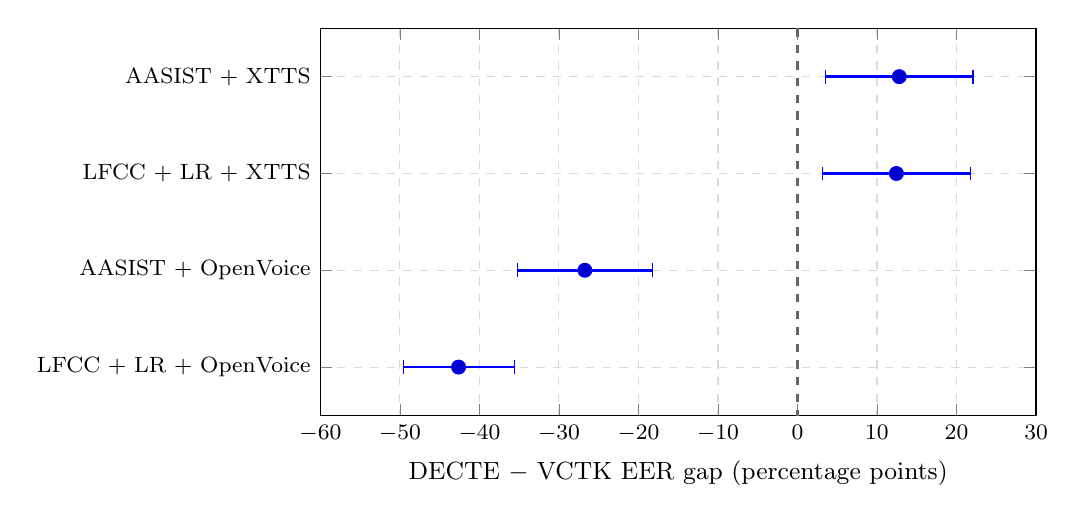
\begin{tikzpicture}
\begin{axis}[
    width=0.88\linewidth,
    height=6.5cm,
    xlabel={DECTE $-$ VCTK EER gap (percentage points)},
    ytick={1,2,3,4},
    yticklabels={AASIST + XTTS,
                 LFCC + LR + XTTS,
                 AASIST + OpenVoice,
                 LFCC + LR + OpenVoice},
    y dir=reverse,
    ymin=0.5, ymax=4.5,
    xmin=-60, xmax=30,
    grid=major, grid style={dashed, gray!30},
    tick label style={font=\footnotesize},
    label style={font=\small},
]
\draw[thick, black!60, dashed] (axis cs:0,0.5) -- (axis cs:0,4.5);
\addplot+[
    only marks,
    mark=*, mark size=2.5pt,
    error bars/.cd,
    x dir=both, x explicit,
    error bar style={line width=1pt},
] coordinates {
    (12.80, 1) +- (9.27, 6.67)
    (12.44, 2) +- (9.32, 10.48)
    (-26.74, 3) +- (8.48, 8.95)
    (-42.62, 4) +- (6.98, 8.16)
};
\end{axis}
\end{tikzpicture}
\caption{DECTE $-$ VCTK EER gaps by generator and detector. Error bars show 95\,\% bootstrap confidence intervals. Positive values mean DECTE is harder than VCTK; negative values mean VCTK is harder. The dashed vertical line marks zero. Both XTTS rows lie entirely above zero (dialect / domain gap); both OpenVoice rows lie entirely below zero (generator-specific corpus interaction).}
\label{fig:gap-direction-forest}
\end{figure}

Two structural properties of this table are worth naming:

\begin{itemize}
    \item \textbf{The XTTS rows (1, 2) are both positive; the OpenVoice rows
        (3, 4) are both negative.} All four gap CIs are entirely on
        their respective sides of zero. The sign split between the two
        generators is not a marginal effect of one detector's noise.
    \item \textbf{Within each generator, the two detectors disagree on absolute
        EER but agree on the sign and rough magnitude of the gap.}
        The magnitude spread is larger for OpenVoice ($-26.74$ vs
        $-42.62$\,pp, $\sim$16\,pp difference) than for XTTS ($+12.80$ vs
        $+12.44$\,pp, $\sim$0.4\,pp difference). For the argument in this
        chapter, only the sign and the 95\,\%-CI-excludes-zero property
        are central.
\end{itemize}


\section{Answers to RQ1, RQ2 and RQ4}
\label{sec:main-results-rq-answers}

Section~\ref{sec:main-results-combined}'s table maps directly onto the three research
questions the chapter set out to address.

\begin{itemize}
    \item \textbf{RQ1 (dialect / domain gap):} \emph{yes, for XTTS.} Under the primary
        detector, the DECTE-vs-VCTK XTTS EER gap is $+12.80$\,pp with 95\,\%
        CI $[+6.13, +22.07]$ (Section~\ref{sec:main-results-aasist-xtts}). Under the second detector, the
        same gap is $+12.44$\,pp with 95\,\% CI $[+1.96, +21.76]$
        (Section~\ref{sec:main-results-lfcc-xtts}). Both intervals lie above zero. Section~\ref{sec:main-results-limitations}
        restates this as a \emph{dialect / domain gap} rather than a pure
        dialect effect.
    \item \textbf{RQ2 (generator dependence):} \emph{yes.} Swapping the generator
        from XTTS v2 to OpenVoice v2, while holding everything else
        fixed, reverses the sign of the DECTE-vs-VCTK EER gap
        (Sections~\ref{sec:main-results-aasist-openvoice}--\ref{sec:main-results-lfcc-openvoice}). The reversal is statistically supported at
        95\,\% on both detectors. This is the strongest quantitative
        argument in the chapter against reading the XTTS result of
        Section~\ref{sec:main-results-aasist-xtts} as evidence that ``DECTE is uniformly harder for
        anti-spoofing''.
    \item \textbf{RQ4 (cross-detector replication):} \emph{yes, for both directions.}
        Both the XTTS DECTE $>$ VCTK gap and the OpenVoice VCTK $>$ DECTE
        reversal reproduce under an architecturally very different
        detector (LFCC + LR) with the same sign and with 95\,\% CIs on
        their respective sides of zero (Sections~\ref{sec:main-results-lfcc-xtts},~\ref{sec:main-results-lfcc-openvoice}). The two
        headline findings of the chapter therefore do not depend on the
        specific AASIST architecture.
\end{itemize}

Put together, these three answers back the thesis' main
descriptive claim about detector behaviour: \textbf{detector reliability
depends jointly on the corpus / domain of the input and on the
generator that produced the spoof.} Neither factor alone
predicts the direction of the observed EER change; only the
combination does.

The chapter does \emph{not} claim, and its evidence does not support,
the stronger reading that dialect alone explains detector
failures. That framing is explicitly ruled out by the OpenVoice
reversal --- under OpenVoice v2, DECTE is the \emph{easier} corpus for
this detector, not the harder one.


\section{Limitations of Chapter 5 results}
\label{sec:main-results-limitations}

Four limitations narrow the scope of the claims in Sections~\ref{sec:main-results-aasist-xtts}--\ref{sec:main-results-rq-answers}.
These are named here so the results can be interpreted correctly;
Chapter~\ref{chap:discussion} treats them at greater length.

\begin{itemize}
    \item \textbf{DECTE and VCTK differ on more than dialect alone.} In
        addition to the dialect axis (Tyneside vs mostly-Southern
        English), the two corpora differ in recording style (interview
        vs studio-read), channel quality (variable field recording vs
        clean studio), age distribution (multi-decade vs concentrated
        in 21--30), and transcript pipeline (Whisper / FairFix vs
        corpus-supplied text). Any ``the detector does worse on DECTE
        than on VCTK'' claim in this chapter should be read as a
        \textbf{dialect / domain gap}, not as evidence of a pure dialect
        effect. Disentangling the dialect axis from the audio-quality
        and demographic axes would require further controls that this
        thesis does not perform (a Northern-English VCTK subset, an
        age-band-matched slice, or a channel-matched noised VCTK).
    \item \textbf{The OpenVoice reversal is a generator-specific corpus
        interaction, not a claim about OpenVoice generally.} The
        observation that OpenVoice v2 produces a stronger detector
        failure on VCTK than on DECTE describes one specific detector-%
        generator-corpus combination. It is not evidence that OpenVoice
        is a ``worse'' or ``more dangerous'' generator in absolute terms
        than XTTS. A different anti-spoofing detector trained on
        OpenVoice-generated data might show a very different pattern.
    \item \textbf{These are detection-performance results, not human-perceptual
        results.} EER measures the operating point at which a
        classifier's false accept rate equals its false reject rate. It
        does not measure how convincing a spoof sounds to a human
        listener, and none of the results in this chapter should be
        read as claims about the naturalness or human-perceptual quality
        of XTTS v2 vs OpenVoice v2 output. That is a separate research
        question not addressed by this thesis.
    \item \textbf{All results are on small held-out slices.} DECTE test:
        $\sim$172 files under the mitigation split, or 216 bonafide + 100
        spoof under the balanced generator comparison. VCTK: 120 unique
        bonafide + 100 spoof per generator, with the two generator
        subsets sharing 80 of 120 source originals (Chapter~\ref{chap:data-methodology}, Section~\ref{sec:methodology-generators-protocol}
        flags this as a \emph{balanced per-generator} comparison, not
        a \emph{fully paired} one). The bootstrap CIs reflect this: they are
        substantially wider than they would be under, say, 1,000-file
        slices. A larger evaluation would produce narrower intervals
        and would allow finer per-subgroup analyses.
\end{itemize}

None of these limitations invalidate the qualitative claims in
Sections~\ref{sec:main-results-aasist-xtts}--\ref{sec:main-results-rq-answers}: the XTTS gap is positive under both detectors,
the OpenVoice gap is negative under both detectors, and both
signs are supported at 95\,\%. What they constrain is how \emph{strongly}
those claims can be phrased in the thesis' broader argument ---
``dialect / domain gap'' rather than ``dialect bias'',
``generator-specific corpus interaction'' rather than ``OpenVoice is
harder in general'', and ``cross-detector replication on the two
detectors tested'' rather than ``architecture-invariant''.
